% Created 2026-11-23 lun 13:05
% Intended LaTeX compiler: pdflatex
\documentclass[a4paper]{article}

\usepackage[utf8]{inputenc}
\usepackage[T1]{fontenc}
\usepackage{graphicx}
\usepackage{longtable}
\usepackage{wrapfig}
\usepackage{rotating}
\usepackage[normalem]{ulem}
\usepackage{amsmath}
\usepackage{amssymb}
\usepackage{capt-of}
\usepackage{hyperref}
\usepackage{color}
\usepackage{listings}
\usepackage[spanish]{babel}
\usepackage[usenames,dvipsnames]{color} % Required for custom colors
\renewcommand{\ttdefault}{pcr} % MONOESPACIO CON NEGRIT
\usepackage{lastpage}
\usepackage{listings}
\usepackage{listingsutf8}
\renewcommand{\lstlistingname}{Listado}
\lstset{frame=single,inputencoding=utf8,basicstyle=\scriptsize\ttfamily,showstringspaces=false,numbers=none}
\definecolor{MyDarkGreen}{rgb}{0.0,0.4,0.0} % This is the color used for comments
\lstset{ breaklines=true, postbreak=\mbox{\textcolor{red}{$\hookrightarrow$}\space}, keywordstyle=\bfseries, keywordstyle=[1]\color{Blue}\bfseries,  keywordstyle=[2]\color{Purple}\bfseries,  keywordstyle=[3]\color{Blue}\underbar,   identifierstyle=,   commentstyle=\usefont{T1}{pcr}{m}{sl}\color{MyDarkGreen}\small,   stringstyle=\color{Purple},   showstringspaces=false,   tabsize=2,   morecomment=[l][\color{Blue}]{...} }
\lstset{literate=  {á}{{\'a}}1 {é}{{\'e}}1 {í}{{\'i}}1 {ó}{{\'o}}1 {ú}{{\'u}}1   {Á}{{\'A}}1 {É}{{\'E}}1 {Í}{{\'I}}1 {Ó}{{\'O}}1 {Ú}{{\'U}}1   {à}{{\`a}}1 {è}{{\`e}}1 {ì}{{\`i}}1 {ò}{{\`o}}1 {ù}{{\`u}}1   {À}{{\`A}}1 {È}{{\'E}}1 {Ì}{{\`I}}1 {Ò}{{\`O}}1 {Ù}{{\`U}}1   {ä}{{\"a}}1 {ë}{{\"e}}1 {ï}{{\"i}}1 {ö}{{\"o}}1 {ü}{{\"u}}1   {Ä}{{\"A}}1 {Ë}{{\"E}}1 {Ï}{{\"I}}1 {Ö}{{\"O}}1 {Ü}{{\"U}}1   {â}{{\^a}}1 {ê}{{\^e}}1 {î}{{\^i}}1 {ô}{{\^o}}1 {û}{{\^u}}1   {Â}{{\^A}}1 {Ê}{{\^E}}1 {Î}{{\^I}}1 {Ô}{{\^O}}1 {Û}{{\^U}}1   {œ}{{\oe}}1 {Œ}{{\OE}}1 {æ}{{\ae}}1 {Æ}{{\AE}}1 {ß}{{\ss}}1   {ű}{{\H{u}}}1 {Ű}{{\H{U}}}1 {ő}{{\H{o}}}1 {Ő}{{\H{O}}}1   {ç}{{\c c}}1 {Ç}{{\c C}}1 {ø}{{\o}}1 {å}{{\r a}}1 {Å}{{\r A}}1   {€}{{\euro}}1 {£}{{\pounds}}1 {«}{{\guillemotleft}}1   {»}{{\guillemotright}}1 {ñ}{{\~n}}1 {Ñ}{{\~N}}1 {¿}{{?`}}1 }
\usepackage{caption}
\usepackage{attachfile2}
\usepackage[margin=1.5cm,includeheadfoot,includehead,includefoot]{geometry}
\hypersetup{colorlinks,linkcolor=black}
\usepackage{fancyhdr}
\pagestyle{fancyplain}
\chead{}
\lhead{}
\rhead{}
\cfoot{}
\lfoot{\begin{footnotesize}alvaro.gonzalezsotillo@educa.madrid.org\end{footnotesize}}
\rfoot{\begin{footnotesize}\thepage / \pageref{LastPage}\end{footnotesize}}
\usepackage[skins]{tcolorbox}
\usepackage{multicol}
\usepackage{changepage} %ajdustwidth
\usepackage{fancybox}
\usepackage{attachfile2}
\lhead{Extraordinaria 2021 (es el \\lhead)}
\rhead{Administración y Gestión de Bases de Datos (es el \\rhead)}
\lhead{Seguridad perimetral}
\rhead{Seguridad y Alta Disponibilidad}
\usepackage{svg}
\usepackage{letltxmacro}
\LetLtxMacro{\originalincludegraphics}{\includegraphics}
\renewcommand{\includegraphics}[2][]{\IfFileExists{#2.pdf}{\originalincludegraphics[#1]{#2.pdf}}{\originalincludegraphics[#1]{#2}}}
\LetLtxMacro{\originalincludesvg}{\includesvg}
\renewcommand{\includesvg}[2][]{\IfFileExists{#2.pdf}{\originalincludegraphics[#1]{#2.pdf}}{\originalincludegraphics[#1]{#2.svg.pdf}}}
\usepackage{comment}
\excludecomment{NOTES}


\date{}
\title{Práctica 04: Cortafuegos con iptables en una topología Docker}
\hypersetup{
 pdfauthor={},
 pdftitle={Práctica 04: Cortafuegos con iptables en una topología Docker},
 pdfkeywords={},
 pdfsubject={},
 pdfcreator={},
 pdflang={Spanish}}
\begin{document}

\maketitle
\tableofcontents

\captionsetup{font=scriptsize}

\textattachfile{/agents/apuntes-clase_gh-pages-llm/seguridad-alta-disponibilidad/apuntes/4/sad-04-practica-iptables-docker.org}{} \vspace{-1em}


\setlength{\parindent}{0em}
\setlength{\parskip}{1em}

\newtcolorbox{Aviso}[1][Aviso]{
  enhanced,
  colback=gray!5!white,
  colframe=gray!75!black,fonttitle=\bfseries,
  colbacktitle=gray!85!black,
  attach boxed title to top left={yshift=-2mm,xshift=2mm},
  title=#1
}

\newtcolorbox{cuadrito}[1][Ignorado]{
  %drop shadow southeast,
  enhanced jigsaw,
  colback=white,
}


\newcommand{\StudentData}{
  \begin{cuadrito}[1\textwidth]
    \vspace{0.3cm}
    \large{
      \textbf{Apellidos:} \hrulefill \\
      \textbf{Nombre:} \hrulefill \\
      \textbf{Fecha:} \hrulefill \hspace{1cm} \textbf{Usuario:} \hrulefill \\
    }
    \vspace{-0.2cm}
  \end{cuadrito}
}

\newcommand{\StudentDataDniFirma}{
  \begin{cuadrito}[1\textwidth]
    \vspace{0.3cm}
    \large{
      \textbf{Apellidos:} \hrulefill \\
      \textbf{Nombre:} \hrulefill  \\
      \textbf{Dni:} \hrulefill \hspace{8cm} \\
      \\
      \textbf{Firma:} \hrulefill \hspace{8cm} \\
    }
    \vspace{-0.2cm}
  \end{cuadrito}
}
\section{Objetivo de la práctica}
\label{sec:org0000000}

Tras la realización de esta práctica, el alumno será capaz de:

\begin{itemize}
\item Comprender la diferencia entre el tráfico \texttt{INPUT}, \texttt{OUTPUT} y \texttt{FORWARD} en un \emph{firewall} Linux.
\item Desplegar con \emph{Docker Compose} una topología con tres redes: una red externa (\texttt{wan}) y dos redes aisladas (\texttt{servers} y \texttt{lan}).
\item Configurar la ruta por defecto de contenedores situados en redes \texttt{internal} para que sus respuestas vuelvan por el router.
\item Publicar un servicio interno hacia la red externa mediante \texttt{DNAT} y \texttt{MASQUERADE} con \texttt{iptables}.
\item Aplicar políticas por defecto restrictivas y reglas de excepción para permitir únicamente el tráfico autorizado.
\item Restringir el acceso a un servicio (\texttt{MySQL}) a un único cliente, e identificar las reglas \texttt{LOG} que registran el resto de intentos.
\item Verificar el aislamiento de las redes, interpretar las tablas de \texttt{iptables} y localizar los mensajes del cortafuegos en el log del kernel del host.
\end{itemize}

Está disponible la \href{https://alvarogonzalezsotillo.github.io/apuntes-clase/seguridad-alta-disponibilidad/apuntes/4/sad-04-practica-iptables-docker.pdf}{última versión de esta práctica en este enlace}.
\section{Descripción del problema}
\label{sec:org0000003}

Se entrega el directorio \texttt{plantilla-practica/} con el escenario ya preparado: \texttt{docker-compose.yml}, \texttt{.env}, los \texttt{Dockerfile} de las imágenes, la página \texttt{http/index.html}, los scripts \texttt{shell-en-*.sh} para entrar en los contenedores y cinco ficheros \texttt{setup.sh} (uno por contenedor) que están prácticamente vacíos.

\textbf{El alumno solo tiene que completar esos ficheros \texttt{setup.sh}.} No hay que modificar el \texttt{docker-compose.yml}, los \texttt{Dockerfile}, el \texttt{.env} ni la página \texttt{index.html}. Cada \texttt{setup.sh} se monta como volumen de solo lectura en \texttt{/setup.sh} y se ejecuta automáticamente al arrancar el contenedor, antes del proceso principal (nginx, MariaDB o \texttt{sleep infinity}). Todas las variables de \texttt{.env} están disponibles dentro de cada contenedor en \texttt{/setup.env}.

La topología es la siguiente:

\begin{center}
\begin{tabular}{llll}
Red & Tipo & Subred & Miembros\\
\hline
\texttt{servers} & \texttt{bridge internal} & \texttt{192.168.52.0/24} & \texttt{router-iptables} (\texttt{eth0}, \texttt{.254}), \texttt{http} (\texttt{.10}), \texttt{mysql} (\texttt{.20})\\
\texttt{lan} & \texttt{bridge internal} & \texttt{192.168.51.0/24} & \texttt{router-iptables} (\texttt{eth1}, \texttt{.254}), \texttt{cliente-admin} (\texttt{.151}), \texttt{cliente} (\texttt{.152})\\
\texttt{wan} & \texttt{bridge} & La asigna Docker & \texttt{router-iptables} (\texttt{eth2}) y el host con Docker\\
\end{tabular}
\end{center}

El comportamiento que se debe conseguir es este:

\begin{itemize}
\item Desde la red \texttt{wan} (por ejemplo, el propio host) se puede acceder al servidor \emph{HTTP} con \texttt{http://<IP-eth2>/}: el router debe redirigir el puerto 80 al contenedor \texttt{http}.
\item Desde la red \texttt{lan}, tanto \texttt{cliente} como \texttt{cliente-admin} pueden acceder a \texttt{http} por HTTP y hacer \texttt{ping} a la red \texttt{servers}.
\item Desde la red \texttt{lan}, \textbf{solo} \texttt{cliente-admin} puede conectarse a \texttt{mysql} por el puerto 3306.
\item Cualquier otro tráfico que atraviese el router se descarta y queda registrado en el log.
\item Ningún contenedor de \texttt{servers} o \texttt{lan} tiene salida directa al exterior: sus rutas por defecto apuntan al router, que es el único paso entre redes.
\end{itemize}

\begin{center}
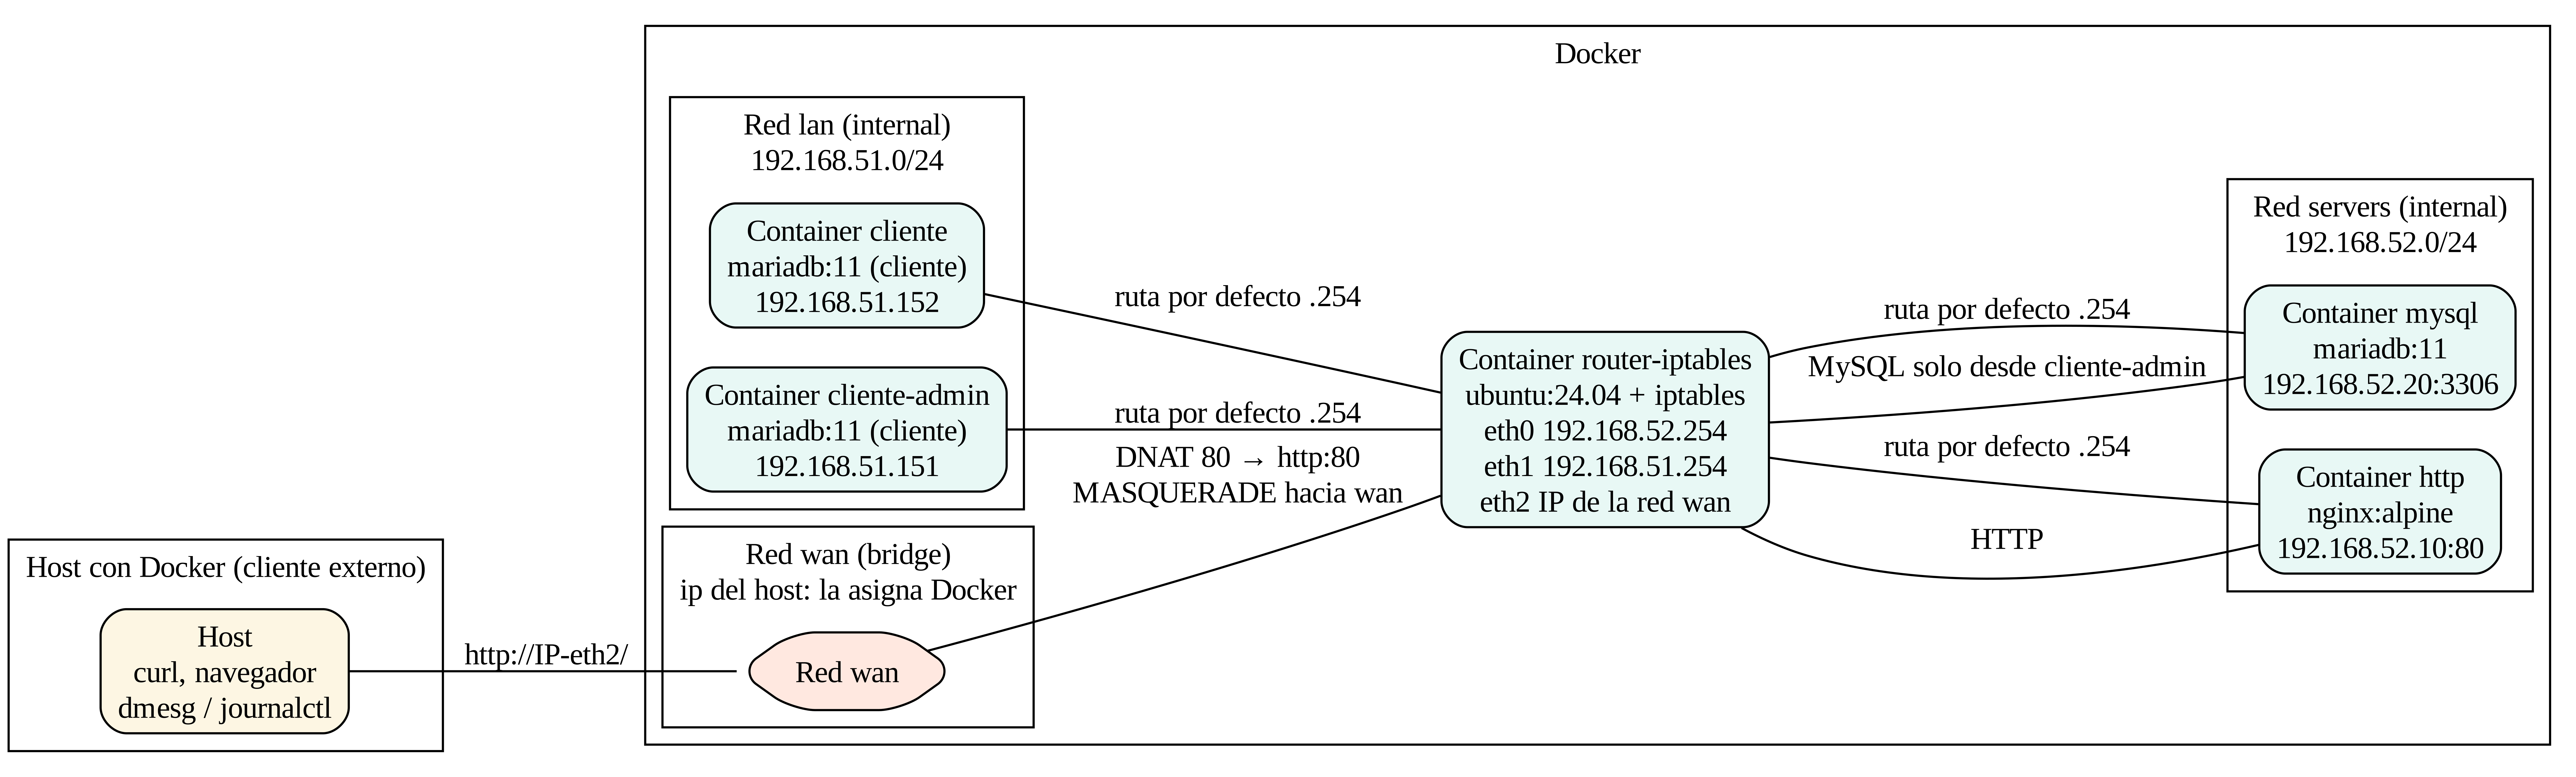
\includegraphics[width=.9\linewidth]{./media/practica-04-topologia-docker.png}
\label{}
\end{center}
\section{Requisitos}
\label{sec:org0000006}

\begin{itemize}
\item Equipo con \emph{Docker} y \emph{Docker Compose} instalados, con permisos para construir imágenes, crear redes y modificar \texttt{sysctl}.
\item Conexión a Internet para construir las imágenes de los \texttt{Dockerfile} (\texttt{ubuntu:24.04}, \texttt{nginx:alpine} y \texttt{mariadb:11}).
\item Un editor de texto para completar los \texttt{setup.sh} y, en el host, \texttt{curl} (o un navegador).
\item Para ver los mensajes de \texttt{iptables -j LOG} hay que desactivar en el host la opción que oculta los logs procedentes de otros espacios de nombres de red:
\end{itemize}

\begin{lstlisting}[language=bash,numbers=none]
sudo sysctl -w net.netfilter.nf_log_all_netns=0
\end{lstlisting}

\begin{itemize}
\item Los ficheros \texttt{setup.sh} deben conservar el permiso de ejecución (\texttt{chmod +x}): son los que ejecuta \texttt{docker-compose.yml} al arrancar cada contenedor.
\end{itemize}
\section{Pasos a seguir}
\label{sec:org000001e}

\subsection{1. Levantar la plantilla sin filtrar nada}
\label{sec:org0000009}

Descomprime (o copia) la plantilla y arranca el escenario. Los \texttt{setup.sh} iniciales solo contienen comentarios, así que en este momento no hay ninguna regla de \texttt{iptables} ni rutas añadidas: sirve para comprobar el punto de partida.

\begin{lstlisting}[language=bash,numbers=none]
cd plantilla-practica
chmod +x */setup.sh
docker compose build
docker compose up -d
docker compose ps
\end{lstlisting}
\subsection{2. Identificar interfaces, direcciones y tablas}
\label{sec:org000000c}

Entra en el router y anota el nombre de cada interfaz, sus IPs, las rutas y el estado del reenvío IP. Compara las tablas de \texttt{iptables} del router con las del host: cada contenedor tiene su propia pila de red.

\begin{lstlisting}[language=bash,numbers=none]
./shell-en-router-iptables.sh
ip -br address
ip route
sysctl net.ipv4.ip_forward
iptables -L -n -v
iptables -t nat -L -n -v
exit
\end{lstlisting}

La red \texttt{wan} no tiene una subred fija en el \texttt{docker-compose.yml}, así que la IP de \texttt{eth2} hay que consultarla en cada arranque:

\begin{lstlisting}[language=bash,numbers=none]
docker exec router-iptables ip -4 -o addr show eth2
\end{lstlisting}

Anota también las IPs del resto de contenedores (\texttt{docker compose ps}) y complétalas en tu diagrama.
\subsection{3. Añadir las rutas por defecto (\texttt{http}, \texttt{mysql}, \texttt{cliente} y \texttt{cliente-admin})}
\label{sec:org000000f}

Las redes \texttt{servers} y \texttt{lan} son \texttt{internal}: \emph{Docker} no les da una ruta por defecto. Un servidor puede responder a otro contenedor de su misma red, pero para responder a clientes de otra red necesita enviar el tráfico al router. Completa los cuatro \texttt{setup.sh} para que lean \texttt{/setup.env} y añadan una ruta por defecto:

\begin{itemize}
\item \texttt{http/setup.sh} y \texttt{mysql/setup.sh} → \texttt{ip route add default via \$SERVERS\_ROUTER\_IP}
\item \texttt{cliente/setup.sh} y \texttt{cliente-admin/setup.sh} → \texttt{ip route add default via \$LAN\_ROUTER\_IP}
\end{itemize}

Comprueba el resultado:

\begin{lstlisting}[language=bash,numbers=none]
docker exec http ip route
docker exec mysql ip route
docker exec cliente ip route
docker exec cliente-admin ip route
docker exec cliente traceroute 192.168.52.10
\end{lstlisting}

El \texttt{traceroute} debe mostrar primero al router (\texttt{192.168.51.254}) y después al servidor \texttt{http}.
\subsection{4. Configurar el cortafuegos del router}
\label{sec:org0000012}

Completa \texttt{router-iptables/setup.sh} (es un script de \emph{bash}) para que, usando las variables de \texttt{/setup.env} en lugar de IPs escritas a mano:

\begin{enumerate}
\item Limpie las tablas \texttt{filter} y \texttt{nat}, dejando antes las políticas en \texttt{ACCEPT} para no quedarse sin acceso durante la limpieza.
\item Establezca \texttt{DROP} como política por defecto de \texttt{INPUT}, \texttt{FORWARD} y \texttt{OUTPUT}, permitiendo el tráfico local por \texttt{lo}.
\item Acepte en \texttt{FORWARD} las conexiones \texttt{ESTABLISHED,RELATED}, para que puedan volver las respuestas de los flujos autorizados.
\item Enmascare con \texttt{MASQUERADE} el tráfico que sale por \texttt{eth2} (red \texttt{wan}).
\item Redirija con \texttt{DNAT} el puerto 80/tcp que llega por \texttt{eth2} hacia \texttt{\$HTTP\_IP:80} y permita ese flujo en \texttt{FORWARD} (\texttt{eth2} → \texttt{eth0}).
\item Permita en \texttt{FORWARD} los paquetes \texttt{ICMP echo-request} que entran por \texttt{eth1} y el HTTP (\texttt{eth1} → \texttt{eth0}, destino \texttt{\$HTTP\_IP}, puerto 80) desde la red \texttt{lan}.
\item Permita MySQL (3306/tcp, destino \texttt{\$MYSQL\_IP}) \textbf{únicamente} cuando el origen sea \texttt{\$CLIENTE\_ADMIN\_IP}.
\item Añada al final reglas \texttt{LOG} con \texttt{-{}-{}limit} para los paquetes descartados en \texttt{INPUT}, \texttt{FORWARD} y \texttt{OUTPUT}, con prefijos reconocibles.
\end{enumerate}

Fíjate en el orden: \texttt{LOG} solo registra, no descarta; las reglas que aceptan tráfico deben ir antes de las reglas de registro, y estas antes de que la política por defecto \texttt{DROP} actúe. El script de ejemplo termina mostrando las reglas con \texttt{watch}; si levantas el escenario con \texttt{-d}, consulta las tablas desde otro terminal con \texttt{docker exec}.
\subsection{5. Volver a aplicar los scripts}
\label{sec:org0000015}

Como los \texttt{setup.sh} se ejecutan al arrancar, después de editarlos hay que recrear los contenedores:

\begin{lstlisting}[language=bash,numbers=none]
docker compose up -d --force-recreate
docker exec router-iptables iptables -L -n -v
docker exec router-iptables iptables -t nat -L -n -v
\end{lstlisting}
\subsection{6. Comprobaciones}
\label{sec:org0000018}

Sustituye \texttt{<IP-eth2>} por la dirección obtenida en el paso 2 (en el bloque siguiente se calcula automáticamente en \texttt{IP\_ETH2}). Rellena una tabla como esta con el resultado real de cada prueba:

\begin{center}
\begin{tabular}{llll}
Origen & Destino & Protocolo & Resultado esperado\\
\hline
host (\texttt{wan}) & \texttt{<IP-eth2>} & TCP 80 & Permitido: página de \texttt{http}\\
host (\texttt{wan}) & \texttt{<IP-eth2>} & ICMP & Bloqueado (política \texttt{INPUT})\\
host (\texttt{wan}) & \texttt{<IP-eth2>} & TCP 3306 & Bloqueado y registrado\\
\texttt{cliente} (\texttt{192.168.51.152}) & \texttt{192.168.52.10} & TCP 80 & Permitido\\
\texttt{cliente} (\texttt{192.168.51.152}) & \texttt{192.168.52.10} & ICMP & Permitido\\
\texttt{cliente} (\texttt{192.168.51.152}) & \texttt{192.168.52.20} & TCP 3306 & Bloqueado y registrado\\
\texttt{cliente-admin} (\texttt{.151}) & \texttt{192.168.52.20} & TCP 3306 & Permitido\\
\texttt{cliente-admin} (\texttt{.151}) & \texttt{192.168.52.10} & TCP 80 & Permitido\\
\end{tabular}
\end{center}

\begin{lstlisting}[language=bash,numbers=none]
# Desde el host: calculamos la IP wan del router
IP_ETH2=$(docker exec router-iptables ip -4 -o addr show eth2 | awk '{print $4}' | cut -d/ -f1)
curl -v http://$IP_ETH2/
ping -c 2 $IP_ETH2
timeout 5 bash -c "cat < /dev/null > /dev/tcp/$IP_ETH2/3306"; echo $?

# Desde los clientes (extra_hosts ya resuelve los nombres http y mysql)
docker exec -it cliente curl -v http://http/
docker exec -it cliente ping -c 2 192.168.52.10
docker exec -it cliente mariadb --connect-timeout=3 -h mysql -u alumno -palumno1234 -e "SELECT 1;"
docker exec -it cliente-admin mariadb --connect-timeout=3 -h mysql -u alumno -palumno1234 -e "SELECT VERSION();"

# Reglas y logs
docker exec router-iptables iptables -L -n -v
docker exec router-iptables iptables -t nat -L -n -v
sudo dmesg -w
# o: sudo journalctl -kf
\end{lstlisting}

En el log deben aparecer mensajes con los prefijos \texttt{IPTABLES INPUT DROP:} e \texttt{IPTABLES FORWARD DROP:} correspondientes a las pruebas bloqueadas. El kernel lo comparten el host y los contenedores, por eso se leen desde el host.
\subsection{7. Cuestiones a responder}
\label{sec:org000001b}

\begin{enumerate}
\item ¿Para qué sirve la ruta por defecto que añades en \texttt{http} y \texttt{mysql}? ¿Qué ocurriría si no la añadieras?
\item ¿Por qué hace falta \texttt{MASQUERADE} en \texttt{eth2} para que funcione el \texttt{DNAT} del puerto 80?
\item Explica la diferencia entre una conexión que termina en \texttt{INPUT} y una que atraviesa \texttt{FORWARD}. ¿Por qué el \texttt{ping} del host al router es bloqueado mientras que el \texttt{ping} de \texttt{cliente} a \texttt{http} es permitido?
\item ¿Qué pasaría si la regla \texttt{LOG} se colocara antes que la regla que acepta a \texttt{cliente-admin}?
\item \texttt{cliente} y \texttt{cliente-admin} están en la misma red. ¿Por qué solo uno de ellos puede conectar con \texttt{mysql}?
\item Si reinicias el contenedor \texttt{router-iptables}, ¿se conservan las reglas? Justifica cómo está resuelto en esta práctica.
\end{enumerate}
\section{Qué se valorará}
\label{sec:org0000021}

Se entregará un documento (\texttt{PDF}, \texttt{ODT} o \texttt{DOCX}) con la siguiente información:

\begin{itemize}
\item \textbf{Topología:} diagrama con las tres redes, contenedores, interfaces, IPs y flujo del tráfico.
\item \textbf{Despliegue:} comandos utilizados y explicación de qué hace cada \texttt{setup.sh} y cuándo se ejecuta.
\item \textbf{Cortafuegos:} relación de reglas aplicadas, explicando la función de cada una y por qué el orden es importante.
\item \textbf{Comprobaciones:} tabla de pruebas permitidas y bloqueadas, salida de \texttt{iptables -L -n -v} y \texttt{iptables -t nat -L -n -v}, y capturas legibles.
\item \textbf{Logs:} captura de los mensajes \texttt{IPTABLES ... DROP} generados por las pruebas fallidas.
\item \textbf{Cuestiones:} respuestas razonadas a las seis preguntas anteriores.
\item \textbf{Claridad y presentación:} pasos ordenados y explicaciones propias.
\end{itemize}
\section{Instrucciones de entrega}
\label{sec:org0000024}

\begin{itemize}
\item \textbf{Modalidad:} individual. Solo se admitirá en pareja si así se indica expresamente en clase.
\item \textbf{Lugar de entrega:} tarea correspondiente a esta práctica en el aula virtual del módulo.
\item \textbf{Contenido:} documento de la práctica y los cinco ficheros \texttt{setup.sh} completados (sin el resto de la plantilla).
\item \textbf{Fecha:} la indicada en el aula virtual.
\end{itemize}
\end{document}
